\documentclass[10pt]{article}
\usepackage[margin=0.9in]{geometry}
\usepackage[T1]{fontenc}
\usepackage{lmodern}
\usepackage{amsmath,amssymb}
\usepackage{booktabs}
\usepackage{graphicx}
\usepackage[numbers,sort&compress]{natbib}
\setlength{\bibsep}{2pt}
\renewcommand{\bibfont}{\footnotesize}
\usepackage{xcolor}
\usepackage{microtype}
\usepackage{xurl}
\usepackage[hidelinks]{hyperref}

% Every measured value in this file is a macro defined in numbers.tex. That file is
% regenerated from results/ by paper/make_numbers.py, and each definition there names the
% artifact it was read from. The comment beside each use below names the same file.
% Generated by paper/make_numbers.py from results/ -- do not edit by hand.
% Each definition names the artifact it was read from.
\newcommand{\ceilTenTwo}{0.4509}% [DERIVED] arithmetic in paper/make_numbers.py
\newcommand{\ceilHundredOneTwo}{0.0688}% [DERIVED] arithmetic in paper/make_numbers.py
\newcommand{\floorTenTwo}{0.7966}% [DERIVED] arithmetic in paper/make_numbers.py
\newcommand{\floorTenSix}{0.0221}% [DERIVED] arithmetic in paper/make_numbers.py
\newcommand{\floorTenTen}{0.0004}% [DERIVED] arithmetic in paper/make_numbers.py
\newcommand{\tminTenExact}{5.142}% [DERIVED] arithmetic in paper/make_numbers.py
\newcommand{\tminTen}{6}% [DERIVED] arithmetic in paper/make_numbers.py
\newcommand{\tminHundredOne}{8}% [DERIVED] arithmetic in paper/make_numbers.py
\newcommand{\ceilEightyIsOne}{1.0}% [DERIVED] arithmetic in paper/make_numbers.py (float64 e^80/(e^80+9) == 1.0)
\newcommand{\ceilTwentyTen}{0.99999998}% [DERIVED] arithmetic in paper/make_numbers.py
\newcommand{\nmSplitTrain}{50{,}000}% results/nmnist_T2_seed0_split.npz
\newcommand{\nmSplitVal}{5{,}000}% results/nmnist_T2_seed0_split.npz
\newcommand{\nmSplitCal}{5{,}000}% results/nmnist_T2_seed0_split.npz
\newcommand{\nmSplitTest}{10{,}000}% results/nmnist_T2_seed0_split.npz
\newcommand{\ncSplitTrain}{5{,}654}% results/ncaltech101_T2_seed0_split.npz
\newcommand{\ncSplitVal}{303}% results/ncaltech101_T2_seed0_split.npz
\newcommand{\ncSplitCal}{1{,}010}% results/ncaltech101_T2_seed0_split.npz
\newcommand{\ncSplitTest}{1{,}742}% results/ncaltech101_T2_seed0_split.npz
\newcommand{\ncSplitTotal}{8{,}709}% results/ncaltech101_T2_seed0_split.npz (sum)
\newcommand{\modelsTotal}{96}% results/*_weights.pt (file count)
\newcommand{\modelsNm}{66}% results/nmnist_*_weights.pt (file count)
\newcommand{\modelsNc}{30}% results/ncaltech101_*_weights.pt (file count)
\newcommand{\hiddenUnits}{256}% results/nmnist_T2_seed0_record.json model_config
\newcommand{\lifTau}{2.0}% results/nmnist_T2_seed0_record.json model_config
\newcommand{\lifThreshold}{1.0}% results/nmnist_T2_seed0_record.json model_config
\newcommand{\surrogateAlpha}{2.0}% results/nmnist_T2_seed0_record.json model_config
\newcommand{\learningRate}{10^{-3}}% results/nmnist_T2_seed0_record.json lr
\newcommand{\batchSize}{128}% results/nmnist_T2_seed0_record.json batch_size
\newcommand{\patienceEpochs}{5}% results/*_record.json epochs_run - best_epoch, less one for the 0-indexed best_epoch in spikecalib/train.py
\newcommand{\epochCap}{50}% results/sweep_nmnist.csv epochs_requested
\newcommand{\epochsMin}{10}% results/sweep_nmnist.csv epochs_run
\newcommand{\epochsMax}{21}% results/sweep_nmnist.csv epochs_run
\newcommand{\nBins}{15}% results/sweep_nmnist.csv n_bins
\newcommand{\nBootstrap}{1{,}000}% results/sweep_nmnist.csv n_bootstrap
\newcommand{\encoderMin}{41}% results/sweep_nmnist.csv encoder_energy_fraction
\newcommand{\encoderMax}{70}% results/sweep_nmnist.csv encoder_energy_fraction
\newcommand{\paramsNmTwo}{1{,}070{,}868}% results/arch_matched.json n_parameters
\newcommand{\paramsNmFour}{375{,}060}% results/arch_matched.json n_parameters
\newcommand{\paramsNcTwo}{2{,}749{,}130}% results/arch_matched.json n_parameters
\newcommand{\paramsNcFour}{464{,}074}% results/arch_matched.json n_parameters
\newcommand{\cellsUnion}{48}% results/readout_experiment.json + caltech_experiment.json + arch_matched.json (count readout)
\newcommand{\cellsSaturated}{45}% results/readout_experiment.json + caltech_experiment.json + arch_matched.json (count readout) |max - ceiling| < 1e-9
\newcommand{\cellsSlack}{3}% results/readout_experiment.json + caltech_experiment.json + arch_matched.json (count readout)
\newcommand{\slackMeanGap}{1.489\times 10^{-3}}% results/readout_experiment.json + caltech_experiment.json + arch_matched.json (count readout)
\newcommand{\cellsMatched}{24}% results/arch_matched.json (count readout)
\newcommand{\matchedMaxDev}{3.83\times 10^{-13}}% results/arch_matched.json
\newcommand{\shareTenTwo}{99.2}% results/conditional_ceiling.json share_explained_theoretical, mean of seeds
\newcommand{\shareTenFour}{90.1}% results/conditional_ceiling.json
\newcommand{\shareTenSix}{44.5}% results/conditional_ceiling.json
\newcommand{\shareHundredOneTwo}{97.1}% results/conditional_ceiling.json
\newcommand{\shareTenTwoFour}{99.3}% results/arch_matched.json share_explained_theoretical
\newcommand{\shareHundredOneTwoTwo}{96.8}% results/arch_matched.json share_explained_theoretical
\newcommand{\eceGapMaxDev}{2\times 10^{-5}}% results/arch_matched.json max |ece - residual|, count readout, T=2
\newcommand{\residTenTwo}{0.5386}% results/conditional_ceiling.json residual
\newcommand{\residHundredOneTwo}{0.3969}% results/conditional_ceiling.json residual
\newcommand{\condGapTenMax}{0.0067}% results/conditional_ceiling.json ceiling_gap_theo_minus_cond, seed means
\newcommand{\condGapTenWorstSeed}{0.0075}% results/conditional_ceiling.json ceiling_gap_theo_minus_cond, single seed
\newcommand{\condGapHundredOneSix}{0.121}% results/conditional_ceiling.json
\newcommand{\condCeilHundredOneSix}{0.6804}% results/conditional_ceiling.json conditional_ceiling_mean
\newcommand{\accHundredOneSix}{0.6427}% results/conditional_ceiling.json test_accuracy
\newcommand{\roCountConfAcc}{$-$0.5386}% results/readout_experiment.json T=2 mean_conf_minus_acc
\newcommand{\roCountEceW}{0.5386}% results/readout_experiment.json T=2 ece_equal_width
\newcommand{\roCountEceM}{0.5386}% results/readout_experiment.json T=2 ece_equal_mass
\newcommand{\roCountLevels}{9}% results/readout_experiment.json T=2 n_distinct
\newcommand{\roCountOps}{9}% results/readout_experiment.json T=2 n_achievable_coverage_levels
\newcommand{\roCountAcc}{0.9850}% results/readout_experiment.json T=2 test_accuracy
\newcommand{\roWcConfAcc}{$-$0.5385}% results/readout_experiment.json T=2 mean_conf_minus_acc
\newcommand{\roWcEceW}{0.5385}% results/readout_experiment.json T=2 ece_equal_width
\newcommand{\roWcEceM}{0.5385}% results/readout_experiment.json T=2 ece_equal_mass
\newcommand{\roWcLevels}{17}% results/readout_experiment.json T=2 n_distinct
\newcommand{\roWcOps}{17}% results/readout_experiment.json T=2 n_achievable_coverage_levels
\newcommand{\roWcAcc}{0.9851}% results/readout_experiment.json T=2 test_accuracy
\newcommand{\roMemConfAcc}{$-$0.0289}% results/readout_experiment.json T=2 mean_conf_minus_acc
\newcommand{\roMemEceW}{0.0290}% results/readout_experiment.json T=2 ece_equal_width
\newcommand{\roMemEceM}{0.0289}% results/readout_experiment.json T=2 ece_equal_mass
\newcommand{\roMemLevels}{9{,}998}% results/readout_experiment.json T=2 n_distinct
\newcommand{\roMemOps}{9{,}998}% results/readout_experiment.json T=2 n_achievable_coverage_levels
\newcommand{\roMemAcc}{0.9851}% results/readout_experiment.json T=2 test_accuracy
\newcommand{\roAccConfAcc}{$+$0.0000}% results/readout_experiment.json T=2 mean_conf_minus_acc
\newcommand{\roAccEceW}{0.0031}% results/readout_experiment.json T=2 ece_equal_width
\newcommand{\roAccEceM}{0.0016}% results/readout_experiment.json T=2 ece_equal_mass
\newcommand{\roAccLevels}{10{,}000}% results/readout_experiment.json T=2 n_distinct
\newcommand{\roAccOps}{10{,}000}% results/readout_experiment.json T=2 n_achievable_coverage_levels
\newcommand{\roAccAcc}{0.9861}% results/readout_experiment.json T=2 test_accuracy
\newcommand{\roAccConfAccSix}{$+$0.0032}% results/readout_experiment.json
\newcommand{\roAccConfAccTen}{$+$0.0047}% results/readout_experiment.json
\newcommand{\roCountOpsExact}{9.3}% results/readout_experiment.json
\newcommand{\leakClosedSix}{53}% results/readout_experiment.json auroc
\newcommand{\leakClosedTen}{62}% results/readout_experiment.json auroc
\newcommand{\ncCountTwoConfAcc}{$-$0.3969}% results/caltech_experiment.json mean_conf_minus_acc
\newcommand{\ncAccTwoConfAcc}{$+$0.0816}% results/caltech_experiment.json mean_conf_minus_acc
\newcommand{\ncCountTwoEceW}{0.3969}% results/caltech_experiment.json
\newcommand{\ncCountTwoEceM}{0.3969}% results/caltech_experiment.json
\newcommand{\ncAccTwoEceW}{0.0826}% results/caltech_experiment.json
\newcommand{\ncAccTwoEceM}{0.0829}% results/caltech_experiment.json
\newcommand{\ncCountTwoAcc}{0.4543}% results/caltech_experiment.json test_accuracy
\newcommand{\ncCountTwoLevels}{132}% results/caltech_experiment.json n_distinct
\newcommand{\ncAccTwoLevels}{1{,}742}% results/caltech_experiment.json n_distinct
\newcommand{\ncCountSixConfAcc}{$-$0.1534}% results/caltech_experiment.json mean_conf_minus_acc
\newcommand{\ncAccSixConfAcc}{$+$0.1843}% results/caltech_experiment.json mean_conf_minus_acc
\newcommand{\ncCountSixEceW}{0.1539}% results/caltech_experiment.json
\newcommand{\ncCountSixEceM}{0.1534}% results/caltech_experiment.json
\newcommand{\ncAccSixEceW}{0.1844}% results/caltech_experiment.json
\newcommand{\ncAccSixEceM}{0.1843}% results/caltech_experiment.json
\newcommand{\ncCountSixAcc}{0.6427}% results/caltech_experiment.json test_accuracy
\newcommand{\ncCountSixLevels}{1{,}180}% results/caltech_experiment.json n_distinct
\newcommand{\ncAccSixLevels}{1{,}742}% results/caltech_experiment.json n_distinct
\newcommand{\ncCountTenConfAcc}{$+$0.0344}% results/caltech_experiment.json mean_conf_minus_acc
\newcommand{\ncAccTenConfAcc}{$+$0.2254}% results/caltech_experiment.json mean_conf_minus_acc
\newcommand{\ncCountTenEceW}{0.0442}% results/caltech_experiment.json
\newcommand{\ncCountTenEceM}{0.0462}% results/caltech_experiment.json
\newcommand{\ncAccTenEceW}{0.2254}% results/caltech_experiment.json
\newcommand{\ncAccTenEceM}{0.2254}% results/caltech_experiment.json
\newcommand{\ncCountTenAcc}{0.6435}% results/caltech_experiment.json test_accuracy
\newcommand{\ncCountTenLevels}{1{,}686}% results/caltech_experiment.json n_distinct
\newcommand{\ncAccTenLevels}{1{,}742}% results/caltech_experiment.json n_distinct
\newcommand{\ncAccMin}{0.4543}% results/caltech_experiment.json test_accuracy
\newcommand{\ncAccMax}{0.6435}% results/caltech_experiment.json test_accuracy
\newcommand{\gainNcFourTwo}{$+$12.82}% results/arch_matched.json test_accuracy (accumulator - count)
\newcommand{\accCountNcFourTwo}{0.4543}% results/arch_matched.json test_accuracy
\newcommand{\accAccumNcFourTwo}{0.5825}% results/arch_matched.json test_accuracy
\newcommand{\gainNcFourSix}{$-$4.52}% results/arch_matched.json test_accuracy (accumulator - count)
\newcommand{\accCountNcFourSix}{0.6427}% results/arch_matched.json test_accuracy
\newcommand{\accAccumNcFourSix}{0.5976}% results/arch_matched.json test_accuracy
\newcommand{\gainNcTwoTwo}{$+$3.08}% results/arch_matched.json test_accuracy (accumulator - count)
\newcommand{\accCountNcTwoTwo}{0.4891}% results/arch_matched.json test_accuracy
\newcommand{\accAccumNcTwoTwo}{0.5199}% results/arch_matched.json test_accuracy
\newcommand{\gainNcTwoSix}{$-$2.24}% results/arch_matched.json test_accuracy (accumulator - count)
\newcommand{\accCountNcTwoSix}{0.5618}% results/arch_matched.json test_accuracy
\newcommand{\accAccumNcTwoSix}{0.5394}% results/arch_matched.json test_accuracy
\newcommand{\gainNmFourTwo}{$-$0.10}% results/arch_matched.json test_accuracy (accumulator - count)
\newcommand{\accCountNmFourTwo}{0.9869}% results/arch_matched.json test_accuracy
\newcommand{\accAccumNmFourTwo}{0.9859}% results/arch_matched.json test_accuracy
\newcommand{\gainNmFourSix}{$-$0.15}% results/arch_matched.json test_accuracy (accumulator - count)
\newcommand{\accCountNmFourSix}{0.9887}% results/arch_matched.json test_accuracy
\newcommand{\accAccumNmFourSix}{0.9872}% results/arch_matched.json test_accuracy
\newcommand{\gainNmTwoTwo}{$+$0.12}% results/arch_matched.json test_accuracy (accumulator - count)
\newcommand{\accCountNmTwoTwo}{0.9850}% results/arch_matched.json test_accuracy
\newcommand{\accAccumNmTwoTwo}{0.9861}% results/arch_matched.json test_accuracy
\newcommand{\gainNmTwoSix}{$-$0.14}% results/arch_matched.json test_accuracy (accumulator - count)
\newcommand{\accCountNmTwoSix}{0.9902}% results/arch_matched.json test_accuracy
\newcommand{\accAccumNmTwoSix}{0.9888}% results/arch_matched.json test_accuracy
\newcommand{\residNcFourSix}{0.1534}% results/arch_matched.json residual
\newcommand{\residNcTwoSix}{0.1159}% results/arch_matched.json residual
\newcommand{\swUncTwoW}{0.5386}% results/sweep_nmnist.csv ece_equal_width
\newcommand{\swUncTwoM}{0.5386}% results/sweep_nmnist.csv ece_equal_mass
\newcommand{\swTempTwoW}{0.0018}% results/sweep_nmnist.csv ece_equal_width
\newcommand{\swTempTwoM}{0.0008}% results/sweep_nmnist.csv ece_equal_mass
\newcommand{\swIsoTwoW}{0.0042}% results/sweep_nmnist.csv ece_equal_width
\newcommand{\swIsoTwoM}{0.0015}% results/sweep_nmnist.csv ece_equal_mass
\newcommand{\swAccTwo}{0.9850}% results/sweep_nmnist.csv test_accuracy
\newcommand{\swUncFourW}{0.1447}% results/sweep_nmnist.csv ece_equal_width
\newcommand{\swUncFourM}{0.1446}% results/sweep_nmnist.csv ece_equal_mass
\newcommand{\swTempFourW}{0.0031}% results/sweep_nmnist.csv ece_equal_width
\newcommand{\swTempFourM}{0.0059}% results/sweep_nmnist.csv ece_equal_mass
\newcommand{\swIsoFourW}{0.0029}% results/sweep_nmnist.csv ece_equal_width
\newcommand{\swIsoFourM}{0.0013}% results/sweep_nmnist.csv ece_equal_mass
\newcommand{\swAccFour}{0.9887}% results/sweep_nmnist.csv test_accuracy
\newcommand{\swUncSixW}{0.0273}% results/sweep_nmnist.csv ece_equal_width
\newcommand{\swUncSixM}{0.0272}% results/sweep_nmnist.csv ece_equal_mass
\newcommand{\swTempSixW}{0.0026}% results/sweep_nmnist.csv ece_equal_width
\newcommand{\swTempSixM}{0.0030}% results/sweep_nmnist.csv ece_equal_mass
\newcommand{\swIsoSixW}{0.0027}% results/sweep_nmnist.csv ece_equal_width
\newcommand{\swIsoSixM}{0.0029}% results/sweep_nmnist.csv ece_equal_mass
\newcommand{\swAccSix}{0.9902}% results/sweep_nmnist.csv test_accuracy
\newcommand{\swUncEightW}{0.0072}% results/sweep_nmnist.csv ece_equal_width
\newcommand{\swUncEightM}{0.0065}% results/sweep_nmnist.csv ece_equal_mass
\newcommand{\swTempEightW}{0.0028}% results/sweep_nmnist.csv ece_equal_width
\newcommand{\swTempEightM}{0.0021}% results/sweep_nmnist.csv ece_equal_mass
\newcommand{\swIsoEightW}{0.0031}% results/sweep_nmnist.csv ece_equal_width
\newcommand{\swIsoEightM}{0.0021}% results/sweep_nmnist.csv ece_equal_mass
\newcommand{\swAccEight}{0.9898}% results/sweep_nmnist.csv test_accuracy
\newcommand{\swUncTenW}{0.0029}% results/sweep_nmnist.csv ece_equal_width
\newcommand{\swUncTenM}{0.0019}% results/sweep_nmnist.csv ece_equal_mass
\newcommand{\swTempTenW}{0.0026}% results/sweep_nmnist.csv ece_equal_width
\newcommand{\swTempTenM}{0.0018}% results/sweep_nmnist.csv ece_equal_mass
\newcommand{\swIsoTenW}{0.0028}% results/sweep_nmnist.csv ece_equal_width
\newcommand{\swIsoTenM}{0.0017}% results/sweep_nmnist.csv ece_equal_mass
\newcommand{\swAccTen}{0.9908}% results/sweep_nmnist.csv test_accuracy
\newcommand{\runsTotal}{15}% results/sweep_nmnist.csv
\newcommand{\straddleW}{13}% results/sweep_nmnist.csv iso_minus_temp_resolvable
\newcommand{\straddleM}{12}% results/sweep_nmnist.csv iso_minus_temp_em_resolvable
\newcommand{\resolveEither}{5}% results/sweep_nmnist.csv (union of resolvable runs)
\newcommand{\resolveBoth}{0}% results/sweep_nmnist.csv (intersection of resolvable runs)
\newcommand{\resWTwoOne}{$+$0.0034}% results/sweep_nmnist.csv paired difference
\newcommand{\resWTwoOneLo}{$+$0.0006}% results/sweep_nmnist.csv interval
\newcommand{\resWTwoOneHi}{$+$0.0044}% results/sweep_nmnist.csv interval
\newcommand{\resWSixZero}{$-$0.0013}% results/sweep_nmnist.csv paired difference
\newcommand{\resWSixZeroLo}{$-$0.0024}% results/sweep_nmnist.csv interval
\newcommand{\resWSixZeroHi}{$-$0.0003}% results/sweep_nmnist.csv interval
\newcommand{\resMFourOne}{$-$0.0044}% results/sweep_nmnist.csv paired difference
\newcommand{\resMFourOneLo}{$-$0.0062}% results/sweep_nmnist.csv interval
\newcommand{\resMFourOneHi}{$-$0.0010}% results/sweep_nmnist.csv interval
\newcommand{\resMFourTwo}{$-$0.0061}% results/sweep_nmnist.csv paired difference
\newcommand{\resMFourTwoLo}{$-$0.0065}% results/sweep_nmnist.csv interval
\newcommand{\resMFourTwoHi}{$-$0.0031}% results/sweep_nmnist.csv interval
\newcommand{\resMEightZero}{$-$0.0009}% results/sweep_nmnist.csv paired difference
\newcommand{\resMEightZeroLo}{$-$0.0014}% results/sweep_nmnist.csv interval
\newcommand{\resMEightZeroHi}{$-$0.0003}% results/sweep_nmnist.csv interval
\newcommand{\isoMinusTempTwoW}{$+$0.0024}% results/sweep_nmnist.csv
\newcommand{\isoMinusTempTwoM}{$+$0.0007}% results/sweep_nmnist.csv
\newcommand{\cellsReadout}{15}% results/readout_experiment.json + caltech_experiment.json + arch_matched.json (count readout)
\newcommand{\cellsCaltech}{9}% results/readout_experiment.json + caltech_experiment.json + arch_matched.json (count readout)
\newcommand{\expectedFalse}{0.75}% [DERIVED] run count in results/sweep_nmnist.csv x 0.05
\newcommand{\nSeeds}{3}% results/sweep_nmnist.csv seed
\newcommand{\splitFingerprint}{e524beccace851af}% results/sweep_nmnist.csv split_fingerprint, seed 0
\newcommand{\ncAccumTwoAcc}{0.5825}% results/caltech_experiment.json test_accuracy
\newcommand{\ncAccumSixAcc}{0.5976}% results/caltech_experiment.json test_accuracy
\newcommand{\ncAccumTenAcc}{0.6072}% results/caltech_experiment.json test_accuracy


\title{Counting Spikes Caps Confidence:\\
A Structural Account of Miscalibration in Low-Timestep Spiking Networks}
\author{Mohammed Abrar Ahasan Chowdhury\\[2pt]
  \small ORCID \href{https://orcid.org/0009-0006-9273-6593}{0009-0006-9273-6593}\\
  \small Independent researcher, Liverpool, United Kingdom\quad \texttt{abrarahasanadil@gmail.com}}
\date{}

\begin{document}
\maketitle

\begin{abstract}
Reading a spiking neural network by counting its output spikes confines its logits to $[0,T]$
for $T$ timesteps, and a softmax over logits in an interval of width $W$ cannot exceed
$e^{W}/(e^{W}+C-1)$ for $C$ classes. The bound is known for normalised and clipped logits.
This paper restates it for spike counts, where the width is the number of timesteps, and
measures what it costs.
Where the cap sits below a model's accuracy it accounts for \shareTenTwo\% ($C=10$, $T=2$) % src: results/conditional_ceiling.json
and \shareHundredOneTwo\% ($C=101$, $T=2$) of expected calibration error before calibration, % src: results/conditional_ceiling.json
under either binning estimator, and for none of it where the cap is slack.
A softmax over firing rates is capped at $e/(e+C-1)$ at every $T$.
A learnable logit scale lifts the cap: it removes the underconfidence on N-MNIST, turns it into
overconfidence on N-Caltech101, and recovers \shareRecovered\% of the accuracy the cap costs there. % src: results/scaled_count_experiment.json
Temperature scaling and isotonic regression tie on N-MNIST, and isotonic regression is better
on N-Caltech101 wherever the cap binds.
A count readout emits at most $\binom{T+C-1}{C-1}$ distinct confidences at any scale, yet on
N-MNIST its few values resolve correct from incorrect predictions as well as an unbounded
readout's.
Of \predictionsNew{} predictions recorded before these experiments, \predictionsHeld{} held and % src: NOTES.md; results/*_experiment.json verdict blocks
\predictionsFalsified{} were falsified. % src: NOTES.md; results/*_experiment.json verdict blocks
\end{abstract}

% =========================================================================================
\section{Introduction}
\label{sec:intro}

A classifier that reports how sure it is can be used more safely than one that does not. A
deployed system can act only when confidence is high, pass uncertain cases to a slower
process, or stop computing once an answer is settled. Each of these needs confidence to mean
what it says: when the model reports 90\%, it should be right about 90\% of the time. A model % illustrative example, not a result
whose confidence matches its accuracy in this way is called calibrated.

Spiking neural networks suit event-driven sensors and low-power hardware because they compute
with sparse binary events spread over time. Every timestep costs latency and energy, so the
pressure in practice is to use as few as possible. That low-timestep regime is also where
spiking networks are reported to be badly calibrated. The natural reading is that such models
are harder to train well.

This paper argues that, for the most common way of reading a spiking network, the problem is
not training. A classifier read out by counting output spikes can only produce whole-number
counts between $0$ and $T$. A softmax over such counts has a hard maximum. When a model is
more accurate than that maximum, no output it can produce is correctly confident, however well
it is trained. The inequality behind this is not new. It is the bound that face-recognition and
out-of-distribution work derived for normalised and clipped logits, with the number of
timesteps in the place of the logit scale (Section~\ref{sec:related}). What has not been done is
to read a spike count as a bounded logit and measure the consequences.

The contributions are five.
\begin{enumerate}
\item A measurement. The known bound, restated for a spike-count readout as
  $e^{T}/(e^{T}+C-1)$, is respected in all \cellsUnion{} count-readout configurations measured, % src: results/readout_experiment.json + caltech_experiment.json + arch_matched.json
  and where it sits below accuracy it accounts for \shareHundredOneTwo\% to \shareTenTwo\% of the % src: results/conditional_ceiling.json
  calibration error before calibration (Sections~\ref{sec:holds} and~\ref{sec:explains}).
\item The rate case. A softmax over firing rates is capped at $e/(e+C-1)$, \rateCeilTen{} for % [DERIVED] paper/make_numbers.py
  ten classes, whatever the number of timesteps (Section~\ref{sec:bound}).
\item A readout taxonomy that is conditional on where the cap sits: below accuracy it forces
  underconfidence, and lifted far above accuracy, by an unbounded readout or by a learned
  scale, it leaves overconfidence on the harder dataset (Section~\ref{sec:readouts}).
\item A comparison of temperature scaling with isotonic regression on spiking networks, to the
  author's knowledge the first, with its predictions recorded in advance. The two tie on
  N-MNIST, isotonic regression is better on N-Caltech101 where the cap binds, and scarce
  calibration data leans towards temperature scaling (Section~\ref{sec:calibrators}).
\item Resolution. A count readout emits at most $\binom{T+C-1}{C-1}$ distinct confidence values
  at any logit scale; temperature scaling cannot change its resolution and isotonic regression
  cannot raise it; and, against a recorded prediction, so few values do not resolve worse than
  an unbounded readout's (Sections~\ref{sec:bound} and~\ref{sec:resolution}).
\end{enumerate}
The last three rest on \predictionsNew{} predictions recorded before the experiments that test % src: NOTES.md
them; \predictionsFalsified{} were falsified, and each is reported as such % src: results/*_experiment.json verdict blocks
(Table~\ref{tab:predictions}).
Code, result artifacts and an interactive view of every number are available at
\url{https://github.com/abrarahasanadil/spikecalib}.

% =========================================================================================
\section{Related work}
\label{sec:related}

This study claims no inequality. The bound of Section~\ref{sec:bound} is a known result,
restated for a readout to which it had not been applied.

\paragraph{The bound, outside spiking networks.}
A softmax over logits confined to an interval cannot reach a probability of one, and
face-recognition work met this when it normalised features and classifier weights. Wang et
al.\ note that cosine logits in $[-1,1]$ cap the correct-class probability at
$e/(e+(n-1)e^{-1})$, ``0.45 when $n=10$'', bound the loss to match, and append a scale layer with
one learnable parameter as the remedy~\citep{wang2017normface}. % [LIT] wang2017normface, Section 3.2 and Proposition 2
Zhang et al.\ state the range for logits in $[0,s]$ as $P\le e^{s}/(e^{s}+C-1)$~\citep{zhang2019adacos}, % [LIT] zhang2019adacos, Eq. (5)
and Wang et al.\ and Ranjan et al.\ invert it into a minimum scale for a target
probability~\citep{wang2018cosface,ranjan2017l2}. % [LIT] wang2018cosface, Eq. (6); ranjan2017l2, Eq. (9)
For normalised logits, Wei et al.\ prove the matching floor on the cross-entropy loss and
remark that it is about 0.7966 at ten classes and unit norm~\citep{wei2022logitnorm}; % [LIT] wei2022logitnorm, Proposition 3.3 and the text after it
for clipped logits they bound the loss by the range $z_{\max}-z_{\min}$~\citep{wei2023logitclip}. % [LIT] wei2023logitclip, Eq. (2) and Proposition 2.1
The two numbers quoted are the ceiling and the loss floor of this study at $T=2$ and $C=10$,
because a spike count over two timesteps and a cosine logit both span an interval of width two.

\paragraph{Scales and readouts in spiking networks.}
Meng et al.\ train directly, take the threshold-weighted firing rate of a spiking output layer
as the network output under a cross-entropy loss, and make the thresholds trainable so that this
rate is not confined to ``a small range''~\citep{meng2022dsr}: a learned scale on a rate % [LIT] meng2022dsr, Section 4.2
readout, given without a bound. Li, Jones and Furber convert trained artificial networks and
keep the output layer at full precision, so the output neurons accumulate input current instead
of spiking, at between about 2.5 and 14 timesteps~\citep{li2023dynamic}. % [LIT] li2023dynamic, as recorded in SOURCES.md
They report confidence that saturates towards 100\% as time passes, and damp it by dividing the
logits by a scalar, which they describe as temperature scaling. That is the unbounded half of % [LIT] li2023dynamic, Section 5.2
the taxonomy in Section~\ref{sec:readouts}, reported independently. Fan et al.\ observe, with a
two-class example, that a rate-decoded output passed through a softmax cannot approach its
label, and train with squared error instead~\citep{fan2024sfod}; their example is an instance % [LIT] fan2024sfod, Section 3.3
of the rate cap of Section~\ref{sec:bound}, given without a formula.

\paragraph{Calibration of spike-count readouts.}
Chen, Park and Simeone use the softmax over spike counts, the readout studied here, to decide
when a directly trained network may stop. They observe that its decisions ``tend to be first
under-confident and then over-confident'' as time passes~\citep{chen2025knowing}, % [LIT] chen2025knowing, Section I and Figure 1(b)
and elsewhere that such networks are overconfident~\citep{chen2024agreeing}; both run for % [LIT] chen2024agreeing
$T=80$ timesteps. Underconfidence of this readout at early timesteps is therefore a published % [LIT] chen2024agreeing: T = 80; chen2025knowing: T = 80
observation, and the bound gives its reason. Read after $t$ steps, a count lies in $[0,t]$, so
the confidence cannot exceed $e^{t}/(e^{t}+C-1)$: for ten classes \ceilTenOne{} after one step, % [DERIVED] paper/make_numbers.py
\ceilTenTwo{} after two and \ceilTenThree{} after three. A network more accurate than that at % [DERIVED] paper/make_numbers.py
those steps is underconfident whatever it has learned. The bound forces the start of the
pattern they report; it does not say where confidence overtakes accuracy. By $t=20$ the ceiling
is \ceilTwentyTen{} and by $t=80$ it is \ceilEightyIsOne{} to double precision, so nothing % [DERIVED] paper/make_numbers.py
holds confidence down. This study measures the early regime directly, at $T=2$ to $10$.

\paragraph{Imposed bounds, and measurement.}
Atarashi et al.\ generalise the softmax to enforce bounds on each output probability and fit
them on a validation set as a remedy for miscalibration~\citep{atarashi2025bounding}. Theirs is % [LIT] atarashi2025bounding
a bound placed on a model; the one studied here is a bound the readout already imposes.
Dimitriadis et al.\ build reliability diagrams and a score decomposition on isotonic
regression, with no binning parameter~\citep{dimitriadis2021stable}; the decomposition used % [LIT] dimitriadis2021stable
here is Murphy's~\citep{murphy1973partition}, which theirs reduces to for discrete forecasts. % [LIT] murphy1973partition; dimitriadis2021stable

% =========================================================================================
\section{The bound, read for spike counts}
\label{sec:bound}

\paragraph{A known lemma.}
Let the logits $z\in\mathbb{R}^{C}$ lie in an interval of width $W$. The largest softmax
probability is $1/\big(1+\sum_{j\ne w}e^{z_j-z_w}\big)$ with $w=\arg\max_j z_j$, and each of the
$C-1$ exponents is at least $-W$, so
\begin{equation}
\label{eq:lemma}
\max_j p_j(z) \;\le\; \frac{e^{W}}{e^{W}+C-1},
\qquad
\mathcal{L}_{\mathrm{CE}} \;\ge\; \ln\!\big(1+(C-1)e^{-W}\big),
\end{equation}
with equality in the first when the winner sits at the top of the interval and every competitor
at the bottom. This is the bound of Zhang et al.\ for logits in $[0,s]$~\citep{zhang2019adacos} % [LIT] zhang2019adacos, Eq. (5)
and, with the loss floor, of Wei et al.\ for normalised and clipped
logits~\citep{wei2022logitnorm,wei2023logitclip}, written for a general interval. % [LIT] wei2022logitnorm, Proposition 3.3; wei2023logitclip, Proposition 2.1

\paragraph{Three readouts, three widths.}
A spike-count readout passes $c\in\{0,1,\dots,T\}^{C}$ to the softmax, where $c_j$ counts the
spikes of output neuron $j$ over $T$ timesteps. Its logits span $[0,T]$, so $W=T$ and
\begin{equation}
\label{eq:ceiling}
p(c) \;\le\; p^{*}(T,C) = \frac{e^{T}}{e^{T}+C-1},
\end{equation}
with equality exactly at the extreme vector $[T,0,\dots,0]$. For $C=10$ and $T=2$ the ceiling
is \ceilTenTwo; with $C=101$ it is \ceilHundredOneTwo. A model that is right on a larger % [DERIVED] paper/make_numbers.py
fraction of its inputs than $p^{*}$ cannot express that accuracy as confidence. Multiplying the
count by a scale $s>0$ gives logits in $[0,sT]$ and a ceiling $e^{sT}/(e^{sT}+C-1)$: the cap
depends on the width $sT$, not on $T$. Dividing the count by $T$ instead, so that the logits are
firing rates in $[0,1]$, gives $W=1$ and
\begin{equation}
\label{eq:rate}
p \;\le\; \frac{e}{e+C-1},
\end{equation}
which is \rateCeilTen{} for ten classes and \rateCeilHundredOne{} for 101, at every $T$. A % [DERIVED] paper/make_numbers.py
softmax over firing rates gains resolution from more timesteps and no confidence at all.
By Equation~\eqref{eq:lemma} the cross-entropy of a count readout cannot fall below
$-\ln p^{*}(T,C)$: for $C=10$, \floorTenTwo{} at $T=2$, \floorTenSix{} at $T=6$ and % [DERIVED] paper/make_numbers.py
\floorTenTen{} at $T=10$. Training losses at different $T$ sit above different floors and % [DERIVED] paper/make_numbers.py
cannot be compared with one another.

\paragraph{A minimum width, and so a minimum scale.}
Requiring the ceiling to reach a target accuracy $a$ gives
\begin{equation}
\label{eq:tmin}
W \;\ge\; \ln\frac{(C-1)\,a}{1-a}, \qquad\text{so}\qquad
T_{\min}(C,a) = \ln\frac{(C-1)\,a}{1-a}\ \ (s=1), \qquad s_{\min} = \frac{T_{\min}(C,a)}{T}.
\end{equation}
The constraint is on the product $sT$. The same expression, for a target class probability,
is the scale bound of Wang et al.\ and of Ranjan et al.~\citep{wang2018cosface,ranjan2017l2}. % [LIT] wang2018cosface, Eq. (6); ranjan2017l2, Eq. (9)
At $a=0.95$ an unscaled ten-class spike-count readout needs $T\ge\tminTen$ % [DERIVED] paper/make_numbers.py
($T_{\min}=\tminTenExact$) to be able to express its own accuracy, and a 101-class readout needs % [DERIVED] paper/make_numbers.py
$T\ge\tminHundredOne$. % [DERIVED] paper/make_numbers.py

\paragraph{The conditional form.}
Equation~\eqref{eq:ceiling} assumes that every competitor is silent. Given the counts the
competitors actually produce on an input, the highest reachable confidence replaces only the
winner's count by $T$:
\begin{equation}
p^{*}_{\mathrm{cond}}(c) = \frac{e^{T}}{e^{T}+\sum_{j\ne w} e^{c_j}} \;\le\; p^{*}(T,C).
\end{equation}
The two coincide when competitors are silent. Over the N-MNIST test inputs the mean
conditional ceiling falls below the theoretical one by at most \condGapTenMax{} averaged over % src: results/conditional_ceiling.json
seeds, and by \condGapTenWorstSeed{} in the worst single seed; on N-Caltech101 at $T=6$, where % src: results/conditional_ceiling.json
many competitors fire, the two differ by \condGapHundredOneSix{} on average. % src: results/conditional_ceiling.json

\paragraph{The scale does not change how many confidences there are.}
Under any scale $s>0$ the confidence of a count vector is
$1/\big(1+\sum_{j\ne w}e^{-s(m-c_j)}\big)$ with $m=\max_j c_j$. It depends only on the multiset
of the $C-1$ gaps $m-c_j$, each an integer in $[0,T]$, so a count readout can emit at most
\begin{equation}
\label{eq:levels}
N(T,C) \;=\; \binom{T+C-1}{C-1}
\end{equation}
distinct confidence values: \levelsTenTwo{} at $T=2$ and $C=10$, \levelsTenFour{} at $T=4$ and % [DERIVED] paper/make_numbers.py
\levelsTenSix{} at $T=6$. Enumerating every count vector at $T=2$, $C=10$ gives exactly % [DERIVED] paper/make_numbers.py; enumeration in tests/test_theory.py
\levelsTenTwo{} values at each of three scales. A scale moves every one of these values and % [DERIVED] tests/test_theory.py
adds none: the cap is set by one number, the count of values only by $T$ and $C$. The bound is
informative only while it is below the number of test samples, which here means $C=10$ and
$T\le6$; at $C=101$ it is already \levelsHundredOneTwo{} at $T=2$. % [DERIVED] paper/make_numbers.py

\paragraph{What a calibrator can do to resolution.}
Group the test samples by their exact confidence value. With $f_k$ the value, $\bar o_k$ the
accuracy and $n_k$ the size of group $k$, and $\bar o$ the overall accuracy, the top-label
Brier score decomposes as~\citep{murphy1973partition} % [LIT] murphy1973partition
\begin{equation}
\label{eq:murphy}
\mathrm{BS} = \underbrace{\sum_k \tfrac{n_k}{n}(f_k-\bar o_k)^2}_{\text{reliability}}
 - \underbrace{\sum_k \tfrac{n_k}{n}(\bar o_k-\bar o)^2}_{\text{resolution}}
 + \underbrace{\bar o(1-\bar o)}_{\text{uncertainty}} .
\end{equation}
Resolution depends on the grouping and not on the values. Temperature scaling changes every
value and keeps the grouping: two samples share a confidence when they share a gap multiset,
at every temperature but the finitely many at which two multisets coincide and their groups
merge. Top-label isotonic regression is a monotone map, so groups can only merge, which cannot
increase a between-group variance. Neither calibrator can add resolution to a count readout.
Keeping the groups is not keeping their order: a two-way tie for first place and a lone winner
one step ahead exchange rank between $s=1$ and $s=0.25$, so the ranking can change under % [DERIVED] tests/test_theory.py
temperature scaling. Where confidences are as many as samples, grouping by exact value says
nothing and bins are needed; the identity then carries two within-bin
terms~\citep{stephenson2008two}, and resolutions are compared only under the same binning. % [LIT] stephenson2008two, Eq. (7)

% =========================================================================================
\section{Method}
\label{sec:method}

\paragraph{Data.}
N-MNIST~\citep{orchard2015converting} has ten classes at $34\times34$ pixels and an official % [LIT] orchard2015converting
test set. Its training set is split into training, validation and calibration sets of
\nmSplitTrain, \nmSplitVal{} and \nmSplitCal{} samples, and it is tested on \nmSplitTest. % src: results/nmnist_T2_seed0_split.npz
N-Caltech101~\citep{orchard2015converting,ncaltech101mirror} has 101 classes and no official % src: results/arch_matched.json n_classes
split. Its \ncSplitTotal{} samples are split into \ncSplitTrain{} for training, % src: results/ncaltech101_T2_seed0_split.npz
\ncSplitVal{} for validation, \ncSplitCal{} for calibration and \ncSplitTest{} for testing, % src: results/ncaltech101_T2_seed0_split.npz
with validation and calibration drawn per class. Its event frames are average-pooled four-fold
to $45\times60$ pixels. % spikecalib/datasets.py: spatial_downsample = 4, spatial = (45, 60)
The calibration set is disjoint from both the validation set and the test set. This is
asserted on the index sets before any calibrator is fitted, because a calibrator scored on the
data it was fitted to reports its own training error. Splits and calibrator fits use CPU
random number generators only, so both reproduce exactly.

\paragraph{Networks.}
All models are convolutional networks of leaky integrate-and-fire neurons built with
SpikingJelly~\citep{fang2023spikingjelly}. The membrane time constant is $\tau=\lifTau$, the % src: results/nmnist_T2_seed0_record.json model_config
threshold \lifThreshold, and the hidden layer has \hiddenUnits{} units. Training uses the ATan % src: results/nmnist_T2_seed0_record.json model_config
surrogate gradient as implemented in SpikingJelly 0.0.0.0.14, % version: pip show spikingjelly
$g'(x)=\alpha/\big(2\,(1+(\tfrac{\pi}{2}\alpha x)^2)\big)$, with $\alpha=\surrogateAlpha$. Two depths are used: two % formula: spikingjelly/activation_based/surrogate.py atan_backward; alpha: results/nmnist_T2_seed0_record.json
convolutional blocks with 32 and 64 channels, and four blocks with 32, 64, 128 and 128. % src: results/arch_matched.json channels
Extra pooling makes the deeper network the smaller one: \paramsNmTwo{} parameters against % src: results/arch_matched.json n_parameters
\paramsNmFour{} on N-MNIST, and \paramsNcTwo{} against \paramsNcFour{} on N-Caltech101. The % src: results/arch_matched.json n_parameters
main N-MNIST experiments use two blocks and the main N-Caltech101 experiments use four. A
matched grid trains both depths on both datasets.

Models are trained with Adam at learning rate $\learningRate$, with batch size \batchSize{} on % optimiser: spikecalib/train.py; lr and batch size: results/nmnist_T2_seed0_record.json
N-MNIST and \batchSizeNc{} on N-Caltech101, % src: results/ncaltech101_T2_seed0_record.json batch_size
for at most \epochCap{} epochs, with early stopping after \patienceEpochs{} epochs without % src: results/sweep_nmnist.csv epochs_requested; results/*_record.json
improvement in validation accuracy. Every run stopped early; the calibration sweep's runs took
\epochsMin--\epochsMax{} epochs. Each configuration is trained at \nSeeds{} seeds, \modelsTotal{} % src: results/sweep_nmnist.csv; results/*_weights.pt
models in all: \modelsNm{} on N-MNIST and \modelsNc{} on N-Caltech101. % src: results/*_weights.pt

\paragraph{Readouts.}
Everything up to the final linear layer is shared; only the aggregation over time differs. The
\emph{count} readout sums the output spikes, $\sum_t s_t$, and is capped by
Equation~\eqref{eq:ceiling}. The \emph{weighted-count} readout computes $\sum_t w_t s_t$ with
weights summing to $T$. It has exactly the same cap but takes many more distinct values, so it
separates the cap from the granularity of the output. The \emph{membrane} readout is a leaky,
non-spiking integrator with the same $\tau$, and it is unbounded. The \emph{accumulator} is the
same integrator with the leak removed, $\sum_t z_t$. It differs from the count readout only by
the spiking threshold, and from the membrane readout only by the leak. The \emph{scaled-count}
readout is the count readout with a learnable logit scale, $s\sum_t s_t$ with
$s=e^{\theta}$ and $\theta$ initialised at zero, so that training starts from the count readout
exactly. The scale is one more parameter, trained by the same optimiser at the same learning
rate. It is the remedy of Wang et al.~\citep{wang2017normface}, used here as a probe of what % [LIT] wang2017normface, Section 3.2
the cap was costing, in three cells: N-MNIST at $T=2$, and N-Caltech101 at $T=2$ and $T=6$.

\paragraph{Calibration and its measurement.}
Two post-hoc calibrators are fitted on the calibration set: temperature scaling, a single scalar
that divides the logits, proposed as a calibrator by Guo et al.~\citep{guo2017calibration}, and
top-label isotonic regression.
They are fitted on both datasets. Expected calibration error (ECE) is the sample-weighted
mean gap between confidence and accuracy over \nBins{} bins, computed with two binning schemes. % src: results/sweep_nmnist.csv n_bins
Equal-width bins are the usual choice, and Guo et al.\ report ECE with 15 of them~\citep{guo2017calibration}. % [LIT] guo2017calibration, Table 1 caption: "ECE (%) (with M = 15 bins)"
A spike-count readout,
however, concentrates its confidences on a few values, which leaves most equal-width bins empty
and can bias the estimate. Equal-mass bins, each holding the same number of samples, do not fail
in that way. Both are reported for every calibration number. The difference between two
calibrators is tested with a paired bootstrap: \nBootstrap{} resamples of the test set, each % src: results/sweep_nmnist.csv n_bootstrap
scoring both calibrators on the same indices, give a 95\% percentile interval on the difference % interval level: spikecalib/calibration.py bootstrap_ece_difference
in ECE. \emph{Two calibrators are said to differ on a run only if that interval excludes zero
under both binning schemes, in the same direction; otherwise they tie.} The two schemes score % rule: NOTES.md, fixed 2026-10-13; spikecalib/calibration.py paired_verdict
identical confidences and differ only in how they bin them, so a difference between calibrators
must appear under both. The rule was fixed before any calibrator was fitted on N-Caltech101.

Where a readout emits few distinct confidence values, the decomposition of
Equation~\eqref{eq:murphy} is computed with no binning at all, by grouping test samples on the
value itself, as Gupta and Ramdas do when estimating the error of discrete-output
predictors~\citep{gupta2022toplabel}. This removes the binning choice, not the finite-sample % [LIT] gupta2022toplabel, Remark 1
bias. For readouts with as many values as samples the bins of each scheme are used instead.

\paragraph{Energy proxy.}
Energy is estimated from synaptic operations. An accumulate costs $E_{\mathrm{AC}}=0.9$\,pJ, % [LIT] horowitz2014energy, Figure 1.1.9
the 32-bit floating-point addition at 45\,nm in Figure~1.1.9 of Horowitz~\citep{horowitz2014energy}, % [LIT] horowitz2014energy, Figure 1.1.9
and a multiply-accumulate $E_{\mathrm{MAC}}=4.6$\,pJ, which is not a figure from that source % [DERIVED] 0.9 + 3.7, SOURCES.md
but the convention of adding its 3.7\,pJ multiplication to the addition. The source calls its % [LIT] horowitz2014energy, Figure 1.1.9
costs rough, so this is a proxy for comparing designs, not a measurement of power. The first
layer receives real-valued frames and performs multiply-accumulates; in the N-MNIST sweep it
accounts for \encoderMin--\encoderMax\% of the modelled energy. % src: results/sweep_nmnist.csv encoder_energy_fraction

% =========================================================================================
\section{Results}
\label{sec:results}

\subsection{The bound holds}
\label{sec:holds}

Two claims are kept apart here. The bound is \emph{respected} when the largest confidence a
model produces never exceeds it. It is \emph{saturated} when the model actually reaches it, to
within $10^{-9}$. % saturation threshold applied in paper/make_numbers.py

A cell is one combination of dataset, architecture, timestep count and seed. Across the
\cellsUnion{} distinct count-readout cells in this study, the bound is respected in all % src: results/readout_experiment.json + caltech_experiment.json + arch_matched.json
\cellsUnion{} and saturated in \cellsSaturated. The N-MNIST readout comparison contributes % src: same union
\cellsReadout{} cells, the N-Caltech101 experiment \cellsCaltech{} and the matched grid % src: results/readout_experiment.json; results/caltech_experiment.json
\cellsMatched; \cellsShared{} of the grid's cells are models it reuses from the other two, and % src: results/arch_matched.json; same union
each is counted once. The \cellsSlack{} cells that are respected but not saturated are all $C=101$, % src: same union
$T=10$, one per seed. There the bound exceeds the largest observed confidence by a mean of % src: same union (slack cells asserted C=101, T=10 in paper/make_numbers.py)
$\slackMeanGap$. Reaching it would need one class to fire at every step while all 100 others % src: same union
stayed silent for all ten.

The matched grid alone, both depths on both datasets at $T\in\{2,6\}$, is \cellsMatched{} % src: results/arch_matched.json
cells. Every one is saturated, and the largest deviation between the observed maximum and the
bound is $\matchedMaxDev$. The bound is a property of the readout, not of a particular % src: results/arch_matched.json
network. Figure~\ref{fig:ceiling} shows it on N-MNIST. The \scRuns{} scaled-count models have % src: results/scaled_count_experiment.json
caps of their own, set by the scale each one learned, and each stays within its cap. % src: results/scaled_count_experiment.json ceiling_signed_excess (asserted below 1e-9 in paper/make_numbers.py)

\begin{figure}[t]
\centering
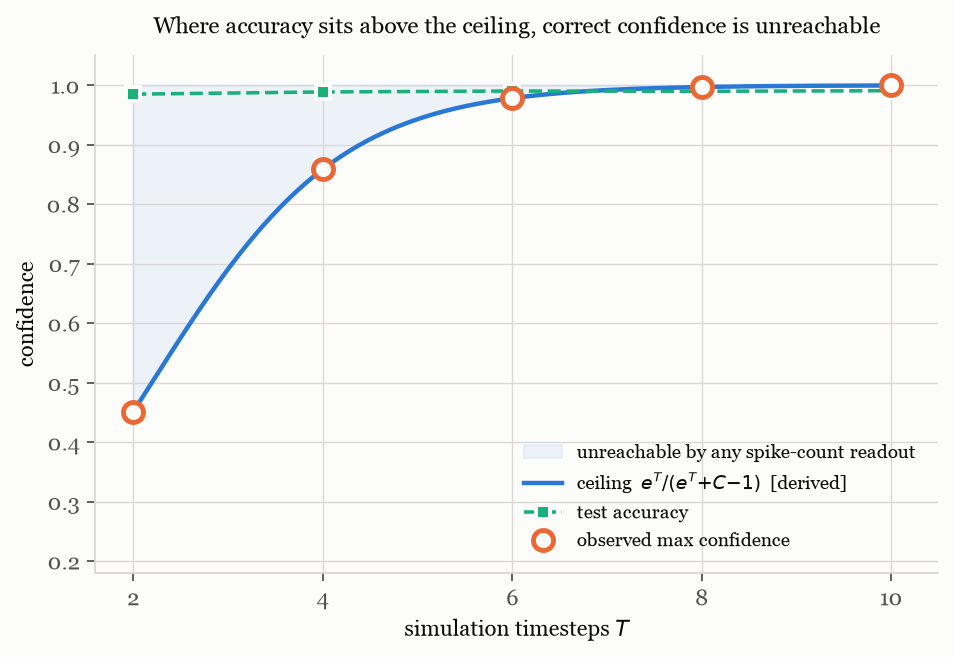
\includegraphics[width=0.56\linewidth]{figures/fig1-ceiling.png} % figures/fig1-ceiling.png, drawn by scripts/make_figures.py from results/readout_stats.json
\caption{The derived ceiling $e^{T}/(e^{T}+C-1)$ for $C=10$, shown against the measured test
accuracy and the largest observed confidence of the N-MNIST count readout (two convolutional
blocks, seed~0). The shaded region is accuracy that no spike-count output can express as confidence.}
\label{fig:ceiling}
\end{figure}

\subsection{Where it binds, it explains the error}
\label{sec:explains}

Let $a$ be accuracy and $\bar p$ mean confidence. Where the ceiling sits below accuracy, no
reachable output can raise mean confidence above $p^{*}$, so at least $a-p^{*}$ of the gap
$a-\bar p$ is forced. The share of the gap that the cap forces is
$\min\{1,\ \max(0,\,a-p^{*})/(a-\bar p)\}$, averaged over seeds.

At $T=2$ this gap is the calibration error. On N-MNIST the gap is \residTenTwo, and ECE is % src: results/conditional_ceiling.json residual
\swUncTwoW{} under equal-width binning and \swUncTwoM{} under equal-mass. On N-Caltech101 the % src: results/sweep_nmnist.csv ece_equal_width, ece_equal_mass
gap is \residHundredOneTwo, and ECE is \ncCountTwoEceW{} and \ncCountTwoEceM{} respectively. % src: results/conditional_ceiling.json; results/caltech_experiment.json
The three agree by construction, not by coincidence. ECE is never smaller than the gap between
accuracy and mean confidence, and it equals that gap when no bin is overconfident, since then no
bin's error offsets another's. Where the cap binds, every confidence lies below the ceiling and
so below the accuracy the bins attain. In every $T=2$ count-readout cell of the matched grid,
both estimators differ from the gap by at most $\eceGapMaxDev$. This is why the shares below % src: results/arch_matched.json ece_equal_width, ece_equal_mass, residual
hold under either binning estimator.

Where the cap binds hardest, it accounts for nearly all
of the error: \shareTenTwo\% on N-MNIST at $T=2$ with two blocks (\shareTenTwoFour\% with % src: results/conditional_ceiling.json; results/arch_matched.json
four), and \shareHundredOneTwo\% on N-Caltech101 at $T=2$ with four blocks % src: results/conditional_ceiling.json
(\shareHundredOneTwoTwo\% with two). On N-MNIST it falls to \shareTenFour\% at $T=4$ and \shareTenSix\% at $T=6$ % src: results/arch_matched.json; results/conditional_ceiling.json
as the ceiling rises towards accuracy. It
is zero wherever the ceiling is slack: at $T=8$ and $10$ on N-MNIST, and at $T=6$ and $10$ on % src: results/conditional_ceiling.json (zero shares asserted in paper/make_numbers.py)
N-Caltech101. Where error remains in those cells, it has some other cause.

\subsection{Where the cap sits sets the direction}
\label{sec:readouts}

Table~\ref{tab:readouts} compares the readouts on identical networks. The taxonomy is
conditional: what decides the direction of miscalibration is whether the cap sits below the
accuracy, not the readout's name. The count readout is underconfident wherever the cap binds. Mean confidence minus accuracy is \roCountConfAcc{} on % src: results/readout_experiment.json
N-MNIST at $T=2$, and \ncCountTwoConfAcc{} and \ncCountSixConfAcc{} on N-Caltech101 at $T=2$ % src: results/caltech_experiment.json
and $T=6$. At $T=10$ on N-Caltech101, where the cap is slack, the same readout is overconfident % src: results/caltech_experiment.json
by \ncCountTenConfAcc. % src: results/caltech_experiment.json

The weighted-count readout isolates the mechanism. It shares the count readout's cap exactly,
but takes \roWcLevels{} distinct confidence values at $T=2$ against \roCountLevels. Its % src: results/readout_experiment.json n_distinct
calibration error does not change: ECE is \roWcEceW{} against \roCountEceW{} under % src: results/readout_experiment.json
equal-width binning, and \roWcEceM{} against \roCountEceM{} under equal-mass. Granularity is % src: results/readout_experiment.json
not the cause. The cap is.

Removing the cap removes the underconfidence and exposes the opposite failure. The accumulator,
which is unbounded and has no leak, is neither over- nor underconfident at $T=2$ on N-MNIST (\roAccConfAcc) and grows % src: results/readout_experiment.json
overconfident with $T$, reaching \roAccConfAccSix{} at $T=6$ and \roAccConfAccTen{} at $T=10$. % src: results/readout_experiment.json
On N-Caltech101 it is overconfident at every $T$ measured: by \ncAccTwoConfAcc, % src: results/caltech_experiment.json
\ncAccSixConfAcc{} and \ncAccTenConfAcc{} at $T=2$, $6$ and $10$. The leaky membrane readout % src: results/caltech_experiment.json
is also unbounded, but it is slightly underconfident, \roMemConfAcc{} at $T=2$. Li et al.\ % src: results/readout_experiment.json
report the unbounded failure independently, with an accumulating readout on converted
networks~\citep{li2023dynamic}.

\begin{table}[t]
\centering
\caption{Readouts, mean over three seeds. Upper: N-MNIST at $T=2$, two convolutional blocks.
Lower: N-Caltech101, four blocks. conf$-$acc is mean confidence minus accuracy; negative values
are underconfident. ECE is given under equal-width (w) and equal-mass (m) binning.}
\label{tab:readouts}
\small
\begin{tabular}{llrrrrr}
\toprule
readout & bound & conf$-$acc & ECE (w) & ECE (m) & distinct values & accuracy \\
\midrule
count          & capped           & \roCountConfAcc & \roCountEceW & \roCountEceM & \roCountLevels & \roCountAcc \\ % src: results/readout_experiment.json
weighted-count & capped           & \roWcConfAcc    & \roWcEceW    & \roWcEceM    & \roWcLevels    & \roWcAcc    \\ % src: results/readout_experiment.json
membrane       & unbounded, leaky & \roMemConfAcc   & \roMemEceW   & \roMemEceM   & \roMemLevels   & \roMemAcc   \\ % src: results/readout_experiment.json
accumulator    & unbounded        & \roAccConfAcc   & \roAccEceW   & \roAccEceM   & \roAccLevels   & \roAccAcc   \\ % src: results/readout_experiment.json
\midrule
readout & $T$ & conf$-$acc & ECE (w) & ECE (m) & distinct values & accuracy \\
\midrule
count       & 2  & \ncCountTwoConfAcc & \ncCountTwoEceW & \ncCountTwoEceM & \ncCountTwoLevels & \ncCountTwoAcc \\ % src: results/caltech_experiment.json
count       & 6  & \ncCountSixConfAcc & \ncCountSixEceW & \ncCountSixEceM & \ncCountSixLevels & \ncCountSixAcc \\ % src: results/caltech_experiment.json
count       & 10 & \ncCountTenConfAcc & \ncCountTenEceW & \ncCountTenEceM & \ncCountTenLevels & \ncCountTenAcc \\ % src: results/caltech_experiment.json
accumulator & 2  & \ncAccTwoConfAcc   & \ncAccTwoEceW   & \ncAccTwoEceM   & \ncAccTwoLevels & \ncAccumTwoAcc \\ % src: results/caltech_experiment.json
accumulator & 6  & \ncAccSixConfAcc   & \ncAccSixEceW   & \ncAccSixEceM   & \ncAccSixLevels & \ncAccumSixAcc \\ % src: results/caltech_experiment.json
accumulator & 10 & \ncAccTenConfAcc   & \ncAccTenEceW   & \ncAccTenEceM   & \ncAccTenLevels & \ncAccumTenAcc \\ % src: results/caltech_experiment.json
\bottomrule
\end{tabular}
\end{table}

\paragraph{Accuracy, and its narrow scope.}
Removing the cap also changes accuracy, but only in a narrow regime. In the matched grid, on
N-Caltech101 at $T=2$, replacing the count readout with the accumulator gains
\gainNcFourTwo{} accuracy points with four convolutional blocks and \gainNcTwoTwo{} % src: results/arch_matched.json
with two. On N-Caltech101 at $T=6$ the same change costs accuracy: \gainNcTwoSix{} points with % src: results/arch_matched.json
two blocks and \gainNcFourSix{} with four. On N-MNIST at $T=2$ it moves accuracy by between % src: results/arch_matched.json
\gainNmFourTwo{} and \gainNmTwoTwo{} points. The direction of the N-Caltech101 gain at $T=2$ % src: results/arch_matched.json
holds at both depths; its size does not.


\paragraph{A learned scale lifts the cap, and overshoots.}
The scaled-count readout asks what the cap alone was costing. Four predictions about it were
recorded before any of its \scRuns{} models was trained (Table~\ref{tab:predictions}). In every % src: results/scaled_count_experiment.json
run the network raised its scale above the minimum of Equation~\eqref{eq:tmin}
(Table~\ref{tab:scaled}), and in all \scRunsStillRising{} it was still rising when early % src: results/scaled_count_experiment.json logit_scale_last_epoch
stopping ended training. On N-MNIST the underconfidence is gone: mean confidence minus accuracy
is \gapScNm{} against \gapCountRefScNm, and ECE is \eceWScNm{} under equal-width binning and % src: results/scaled_count_experiment.json
\eceMScNm{} under equal-mass, with accuracy \accDeltaScNm{} points relative to the count readout. % src: results/scaled_count_experiment.json
The number of distinct confidence values is unchanged, \levelsMinScNm{} to \levelsMaxScNm, as % src: results/scaled_count_experiment.json n_distinct
Equation~\eqref{eq:levels} requires.

On N-Caltech101 the scale does not calibrate. It changes the sign. Mean confidence minus
accuracy is \gapScNcTwo{} at $T=2$ and \gapScNcSix{} at $T=6$, positive in all \scRunsNc{} runs. % src: results/scaled_count_experiment.json
At $T=6$ neither ceiling binds, and the count readout's underconfidence of \residNcFourSix{} was % src: results/arch_matched.json
the study's largest unexplained quantity. Freeing the logit range removes it, so it is an effect
of the bounded range on what the network learns and not something the bound forces. What
replaces it is overconfidence of similar size, and accuracy changes by \accDeltaScNcSix{} points. % src: results/scaled_count_experiment.json
A cap far above the accuracy, whether the readout is unbounded or its scale was learned, leaves
the model overconfident on this dataset in every run measured.

At $T=2$ on N-Caltech101 the scale recovers part of the accuracy the cap costs: the
scaled-count readout reaches \accScNcTwo, between the count readout's \accCountRefScNcTwo{} and % src: results/scaled_count_experiment.json
the accumulator's \accAccumRefScNcTwo, or \shareRecovered\% of the gap. The prediction was at % src: results/scaled_count_experiment.json predictions.7
least half, and it is \verdictSeven. % src: results/scaled_count_experiment.json predictions.7

\begin{table}[t]
\centering
\caption{The scaled-count readout, mean over three seeds; scale and $s_{\min}$ are ranges over
seeds. $s_{\min}$ uses each run's own test accuracy. conf$-$acc is mean confidence minus
accuracy before any calibrator.}
\label{tab:scaled}
\small
\begin{tabular}{lcccrrrrrr}
\toprule
 & & & & \multicolumn{3}{c}{conf$-$acc} & \multicolumn{3}{c}{accuracy} \\
\cmidrule(lr){5-7}\cmidrule(lr){8-10}
dataset & $T$ & learned $s$ & $s_{\min}$ & count & scaled & accum. & count & scaled & accum. \\
\midrule
N-MNIST      & 2 & \scaleMinScNm--\scaleMaxScNm       & \sminMinScNm--\sminMaxScNm       & \gapCountRefScNm    & \gapScNm    & \gapAccumRefScNm    & \accCountRefScNm    & \accScNm    & \accAccumRefScNm    \\ % src: results/scaled_count_experiment.json
N-Caltech101 & 2 & \scaleMinScNcTwo--\scaleMaxScNcTwo & \sminMinScNcTwo--\sminMaxScNcTwo & \gapCountRefScNcTwo & \gapScNcTwo & \gapAccumRefScNcTwo & \accCountRefScNcTwo & \accScNcTwo & \accAccumRefScNcTwo \\ % src: results/scaled_count_experiment.json
N-Caltech101 & 6 & \scaleMinScNcSix--\scaleMaxScNcSix & \sminMinScNcSix--\sminMaxScNcSix & \gapCountRefScNcSix & \gapScNcSix & \gapAccumRefScNcSix & \accCountRefScNcSix & \accScNcSix & \accAccumRefScNcSix \\ % src: results/scaled_count_experiment.json
\bottomrule
\end{tabular}
\end{table}

\begin{table}[t]
\centering
\caption{Predictions recorded before the corresponding runs, with the condition each had to
meet and what was measured. Gaps are mean confidence minus accuracy; ``tie'' and ``differ''
follow the rule of Section~\ref{sec:method}.}
\label{tab:predictions}
\small
\begin{tabular}{lp{0.47\linewidth}p{0.25\linewidth}l}
\toprule
 & prediction & measured & outcome \\
\midrule
6a & N-MNIST, $T=2$: scaled-count $|\text{gap}|<0.05$ & \gapScNm & \verdictSixA \\ % threshold: NOTES.md prediction 6a; src: results/scaled_count_experiment.json
6b & N-Caltech101, $T=2$: scaled-count gap above 0 & \gapScNcTwo & \verdictSixB \\ % threshold: NOTES.md prediction 6b; src: results/scaled_count_experiment.json
7 & N-Caltech101, $T=2$: scaled-count accuracy at least \thresholdSeven, half the gap to the accumulator & \accScNcTwo{} (\shareRecovered\% of the gap) & \verdictSeven \\ % src: results/scaled_count_experiment.json
8 & N-Caltech101, $T=6$: scaled-count gap above $-0.05$ & \gapScNcSix & \verdictEight \\ % threshold: NOTES.md prediction 8; src: results/scaled_count_experiment.json
9 & N-MNIST, $T=2$: count resolution below the accumulator's in all \nineTotal{} comparisons & below in \nineBelow{} & \verdictNine \\ % src: results/resolution_experiment.json
10 & N-Caltech101: calibrators tie in at least 7 of 9 count runs & tie in \ncTies{} & \verdictTen \\ % threshold: NOTES.md prediction 10; src: results/caltech_calibrators.json
11 & N-MNIST, $T=2$, 100 calibration samples: temperature better in at least 10 of \csDraws{} draws for 2 of 3 seeds; ties at 1,000 and 5,000 & at most \csTempWinsMaxHundred{} of \csDraws{} in any seed; ties at both & \verdictEleven \\ % thresholds and sizes: NOTES.md prediction 11; src: results/calibration_size_experiment.json
\bottomrule
\end{tabular}
\end{table}

\begin{figure}[t]
\centering
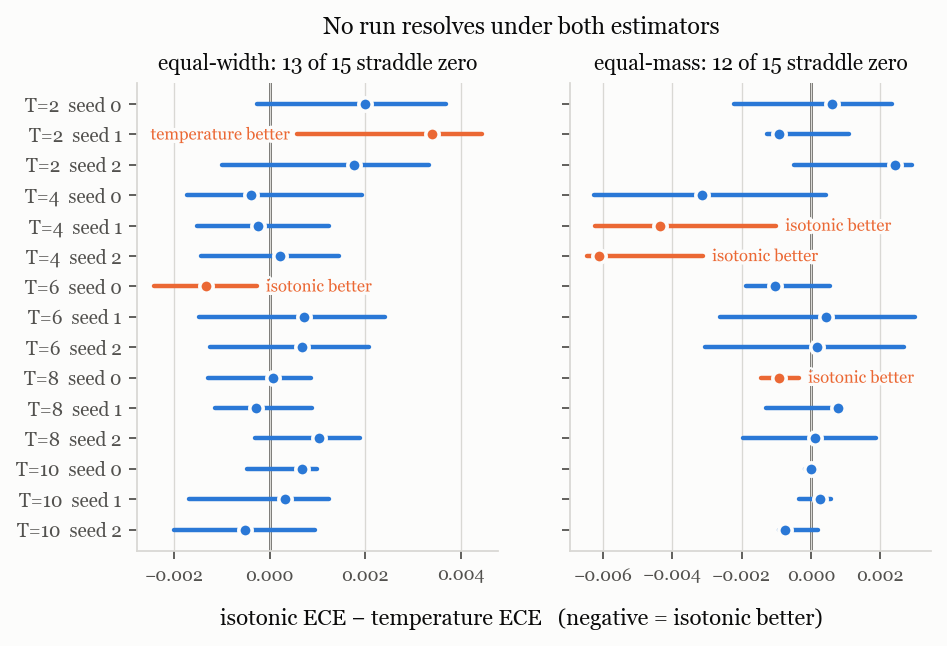
\includegraphics[width=0.66\linewidth]{figures/fig4-paired-difference.png} % figures/fig4-paired-difference.png, drawn by spikecalib/figures.py from results/sweep_nmnist.csv
\caption{Isotonic minus temperature ECE with its paired 95\% bootstrap interval, for every % src: results/sweep_nmnist.csv
N-MNIST run (two convolutional blocks). Left: equal-width binning, where \straddleW{} of % src: results/sweep_nmnist.csv iso_minus_temp_resolvable
\runsTotal{} intervals straddle zero. Right: equal-mass binning, where \straddleM{} of % src: results/sweep_nmnist.csv iso_minus_temp_em_resolvable
\runsTotal{} do. The panels share rows but not horizontal scales. Orange marks an interval
that excludes zero; \resolveBoth{} of \runsTotal{} rows are orange in both panels.} % src: results/sweep_nmnist.csv
\label{fig:paired}
\end{figure}

\subsection{The choice of calibrator depends on the regime}
\label{sec:calibrators}

The following prediction was recorded on 2026-09-10, before any calibrator was fitted to a % NOTES.md, "Pre-registered prediction, recorded 2026-09-10"
trained model. It was based on the measured distribution of the count readout's confidences on
N-MNIST, and it is quoted as written:
\begin{quote}
\emph{Temperature scaling will match or beat top-label isotonic at every $T$, and the isotonic
advantage will not be statistically resolvable at any $T$ --- that is, the 95\% % NOTES.md, quoted verbatim
paired-bootstrap interval on the equal-width ECE difference will straddle zero at $T$ in
$\{2, 4, 6, 8, 10\}$.} % NOTES.md, quoted verbatim
\end{quote}
It ran against the study's own starting hypothesis, which held that isotonic regression's extra
capacity would beat a single temperature by a margin that grows as $T$ falls.

Table~\ref{tab:calibrators} gives the result. Calibration matters a great deal at low $T$. At
$T=2$ it takes ECE from \swUncTwoW{} to \swTempTwoW{} under equal-width binning, and from % src: results/sweep_nmnist.csv
\swUncTwoM{} to \swTempTwoM{} under equal-mass binning. Which calibrator is used matters much % src: results/sweep_nmnist.csv
less. Under equal-width binning, \straddleW{} of \runsTotal{} paired intervals straddle zero. Under % src: results/sweep_nmnist.csv
equal-mass binning, \straddleM{} of \runsTotal{} do. % src: results/sweep_nmnist.csv

\paragraph{Outcome of the prediction.}
As written, the prediction is false. Under equal-width binning, the estimator it named, isotonic
regression beats temperature scaling resolvably at $T=6$, seed~0. Its substance, that the two % src: results/sweep_nmnist.csv iso_minus_temp_resolvable
calibrators tie, holds. The study's own hypothesis fares worse. At $T=2$, the most discrete
regime, temperature scaling beats isotonic regression on average, by \isoMinusTempTwoW{} under % src: results/sweep_nmnist.csv
equal-width binning and \isoMinusTempTwoM{} under equal-mass. % src: results/sweep_nmnist.csv

\paragraph{The runs that resolve are disjoint.}
Under equal-width binning the resolvable runs are $T=2$ seed~1, favouring temperature scaling, % src: results/sweep_nmnist.csv iso_minus_temp_resolvable
and $T=6$ seed~0, favouring isotonic regression. Under equal-mass binning they are $T=4$ seeds~1 % src: results/sweep_nmnist.csv iso_minus_temp_resolvable, iso_minus_temp_em_resolvable
and~2 and $T=8$ seed~0, all favouring isotonic regression (Table~\ref{tab:calibrators}, lower; % src: results/sweep_nmnist.csv iso_minus_temp_em_resolvable
Figure~\ref{fig:paired}). \resolveEither{} runs resolve under one estimator or the other and % src: results/sweep_nmnist.csv
\resolveBoth{} under both. That disjointness, not either count, is the evidence. The two % src: results/sweep_nmnist.csv
estimators score identical confidences and differ only in how they bin them, so a run in which
the calibrators genuinely differed would resolve under both, in the same direction. None does,
and \runsTotal{} intervals at a 95\% level would yield about \expectedFalse{} such runs per % [DERIVED] paper/make_numbers.py
estimator by chance alone. On N-MNIST, with \nmSplitCal{} calibration samples, the choice % src: results/nmnist_T2_seed0_split.npz
between the two does not matter. This reasoning is the rule of Section~\ref{sec:method}, under
which all \runsTotal{} runs are ties; it was fixed before being applied to anything else. % src: results/sweep_nmnist.csv

\paragraph{On N-Caltech101 it matters.}
The prediction, recorded before any calibrator was fitted on this dataset, was that the two
would tie in at least seven of the nine count-readout runs. They tie in \ncTies. In the other % src: results/caltech_calibrators.json prediction_10
\ncDiffer, isotonic regression is better under both estimators (Table~\ref{tab:caltechcal}): % src: results/caltech_calibrators.json
all three seeds at $T=2$, and \ncDifferSix{} of three at $T=6$. At $T=2$ temperature scaling % src: results/caltech_calibrators.json
takes ECE from \ccUncTwoW{} to \ccTempTwoW{} under equal-width binning and \ccTempTwoM{} under % src: results/caltech_calibrators.json
equal-mass, and isotonic regression takes it to \ccIsoTwoW{} and \ccIsoTwoM. The fitted % src: results/caltech_calibrators.json
temperature there is \ccTemperatureTwo, a scale above $s_{\min}$, so the cap is lifted; the % src: results/caltech_calibrators.json temperature
error that remains is one that no single scale removes. At $T=10$, where the cap is slack, the
calibrators tie in all three runs. The study's starting hypothesis, that isotonic regression
gains on a single temperature as $T$ falls, fails on N-MNIST and is the pattern of these nine
runs on N-Caltech101. The calibration set here is \ccCalSize{} samples, ten per class, and the test set % src: results/caltech_calibrators.json n_cal
\ccTestSize, so the result rests on nine runs of one architecture. % src: results/caltech_calibrators.json n_test

Calibrators were also fitted to the unbounded readouts on this dataset. For the accumulator the
two differ in \ccAccumDiffer{} of \ccAccumRuns{} runs, each time in favour of isotonic % src: results/caltech_calibrators.json paired, accumulator
regression. For the scaled-count readout, of \ccScaledRuns{} runs, \ccScaledTie{} tie, % src: results/caltech_calibrators.json paired, scaled-count
\ccScaledTemp{} favour temperature scaling and \ccScaledIso{} favours isotonic regression. % src: results/caltech_calibrators.json paired, scaled-count

\paragraph{With little calibration data it leans the other way.}
On N-MNIST at $T=2$ the calibration set was subsampled to 100 and to 1,000 samples, % sizes: NOTES.md, prediction 11
\csDraws{} stratified draws per seed and size. With 100 samples temperature scaling is better % src: results/calibration_size_experiment.json draws
in \csTempWinsHundred{} of \csDrawsTotal{} draws and isotonic regression in \csIsoWinsHundred; % src: results/calibration_size_experiment.json summary
with 1,000 the counts are \csTempWinsThousand{} and \csIsoWinsThousand; with all % src: results/calibration_size_experiment.json summary
\nmSplitCal{} they are \csTempWinsFull{} and \csIsoWinsFull. Mean ECE at 100 samples is % src: results/calibration_size_experiment.json summary
\csTempWHundred{} for temperature scaling against \csIsoWHundred{} for isotonic regression % src: results/calibration_size_experiment.json rows
under equal-width binning, and \csTempMHundred{} against \csIsoMHundred{} under equal-mass. % src: results/calibration_size_experiment.json rows
The direction is the expected one for a method with one parameter. The prediction asked for
more: temperature scaling better in at least half the draws for two of three seeds. No seed
reaches half, the largest being \csTempWinsMaxHundred{} of \csDraws, so it is \verdictEleven. % src: results/calibration_size_experiment.json prediction_11


\begin{table}[t]
\centering
\caption{Calibrators on N-MNIST, two convolutional blocks, mean over three seeds. Upper: ECE
under equal-width (w) and equal-mass (m) binning. Lower: every run whose paired 95\% interval % interval level: spikecalib/calibration.py bootstrap_ece_difference
on isotonic minus temperature ECE excludes zero; negative favours isotonic regression.}
\label{tab:calibrators}
\small
\begin{tabular}{rrcccccc}
\toprule
 & & \multicolumn{2}{c}{uncalibrated} & \multicolumn{2}{c}{temperature} & \multicolumn{2}{c}{isotonic} \\
\cmidrule(lr){3-4}\cmidrule(lr){5-6}\cmidrule(lr){7-8}
$T$ & accuracy & w & m & w & m & w & m \\
\midrule
2  & \swAccTwo   & \swUncTwoW   & \swUncTwoM   & \swTempTwoW   & \swTempTwoM   & \swIsoTwoW   & \swIsoTwoM   \\ % src: results/sweep_nmnist.csv
4  & \swAccFour  & \swUncFourW  & \swUncFourM  & \swTempFourW  & \swTempFourM  & \swIsoFourW  & \swIsoFourM  \\ % src: results/sweep_nmnist.csv
6  & \swAccSix   & \swUncSixW   & \swUncSixM   & \swTempSixW   & \swTempSixM   & \swIsoSixW   & \swIsoSixM   \\ % src: results/sweep_nmnist.csv
8  & \swAccEight & \swUncEightW & \swUncEightM & \swTempEightW & \swTempEightM & \swIsoEightW & \swIsoEightM \\ % src: results/sweep_nmnist.csv
10 & \swAccTen   & \swUncTenW   & \swUncTenM   & \swTempTenW   & \swTempTenM   & \swIsoTenW   & \swIsoTenM   \\ % src: results/sweep_nmnist.csv
\end{tabular}

\vspace{6pt}
\begin{tabular}{lrrrc}
\toprule
estimator & $T$ & seed & isotonic $-$ temperature & 95\% interval \\ % interval level: spikecalib/calibration.py bootstrap_ece_difference
\midrule
equal-width & 2 & 1 & \resWTwoOne    & [\resWTwoOneLo, \resWTwoOneHi]       \\ % src: results/sweep_nmnist.csv
equal-width & 6 & 0 & \resWSixZero   & [\resWSixZeroLo, \resWSixZeroHi]     \\ % src: results/sweep_nmnist.csv
equal-mass  & 4 & 1 & \resMFourOne   & [\resMFourOneLo, \resMFourOneHi]     \\ % src: results/sweep_nmnist.csv
equal-mass  & 4 & 2 & \resMFourTwo   & [\resMFourTwoLo, \resMFourTwoHi]     \\ % src: results/sweep_nmnist.csv
equal-mass  & 8 & 0 & \resMEightZero & [\resMEightZeroLo, \resMEightZeroHi] \\ % src: results/sweep_nmnist.csv
\bottomrule
\end{tabular}
\end{table}

\begin{table}[t]
\centering
\caption{Calibrators on the N-Caltech101 count readout, four convolutional blocks, mean over
three seeds. ECE under equal-width (w) and equal-mass (m) binning. ``differ'' counts the seeds
in which the calibrators differ under the rule of Section~\ref{sec:method}; every such run
favours isotonic regression.}
\label{tab:caltechcal}
\small
\begin{tabular}{rrccccccc}
\toprule
 & & \multicolumn{2}{c}{uncalibrated} & \multicolumn{2}{c}{temperature} & \multicolumn{2}{c}{isotonic} & \\
\cmidrule(lr){3-4}\cmidrule(lr){5-6}\cmidrule(lr){7-8}
$T$ & accuracy & w & m & w & m & w & m & differ \\
\midrule
2  & \ccAccTwo & \ccUncTwoW & \ccUncTwoM & \ccTempTwoW & \ccTempTwoM & \ccIsoTwoW & \ccIsoTwoM & \ncDifferTwo{} of 3 \\ % src: results/caltech_calibrators.json
6  & \ccAccSix & \ccUncSixW & \ccUncSixM & \ccTempSixW & \ccTempSixM & \ccIsoSixW & \ccIsoSixM & \ncDifferSix{} of 3 \\ % src: results/caltech_calibrators.json
10 & \ccAccTen & \ccUncTenW & \ccUncTenM & \ccTempTenW & \ccTempTenM & \ccIsoTenW & \ccIsoTenM & \ncDifferTen{} of 3 \\ % src: results/caltech_calibrators.json
\bottomrule
\end{tabular}
\end{table}

\subsection{Resolution}
\label{sec:resolution}

\paragraph{The count of confidence values.}
Whether observed confidences respect Equation~\eqref{eq:levels} could be read from results that
existed before the bound was derived, so it is reported as a check and not a prediction. In all
\checkCells{} count and scaled-count cells the number of distinct confidences is within the % src: results/resolution_experiment.json check
bound. In the \checkInformative{} cells where the bound is below the number of test samples, % src: results/resolution_experiment.json check
the models use at most \shareOfBoundMax\% of it: on N-MNIST at $T=2$, between % src: results/resolution_experiment.json check rows
\levelsObsMinNmTwo{} and \levelsObsMaxNmTwo{} values of a possible \levelsTenTwo, with or % src: results/resolution_experiment.json check rows
without the learned scale.

\paragraph{Few values do not mean low resolution.}
The prediction was that on N-MNIST at $T=2$, where the count readout and the accumulator have
the same accuracy, the count readout's resolution term would be below the accumulator's under
both binning schemes, with and without the learned scale and after either calibrator: twelve
comparisons. It is \verdictNine: the count readout is below in \nineBelow{} of \nineTotal. % src: results/resolution_experiment.json prediction_9
Under equal-width binning its resolution is \resCountW{} against the accumulator's \resAccumW, % src: results/resolution_experiment.json
which is \resRatioCountW{} and \resRatioAccumW{} of their uncertainty terms. Under equal-mass % src: results/resolution_experiment.json res_over_unc
binning the count readout's confidences fall into a single bin in every seed, so its resolution
there is zero by construction (\resCountM{} against \resAccumM); \nineBelowDegenerate{} of the % src: results/resolution_experiment.json
\nineBelow{} comparisons that go the predicted way are of this kind. With the learned scale the count readout is above
the accumulator in all six comparisons (\resScaledW{} under equal-width), partly because its % src: results/resolution_experiment.json
lower accuracy leaves more to resolve. Between \levelsObsMinNmTwo{} and \levelsObsMaxNmTwo{} % src: results/resolution_experiment.json check rows
confidence values separate right from wrong, in the Brier sense, as well as the accumulator's
\roAccLevels{} do. What the count readout gives up is
ranking: the area under the ROC curve of confidence for correctness is \aurocCountNmTwo{} % src: results/resolution_experiment.json auroc
against \aurocAccumNmTwo. On N-Caltech101, where accuracies differ and no prediction was made, % src: results/resolution_experiment.json auroc
resolution as a share of uncertainty at $T=2$ is \ncResRatioCountM, \ncResRatioScaledM{} and % src: results/resolution_experiment.json res_over_unc
\ncResRatioAccumM{} for the count, scaled-count and accumulator readouts under equal-mass % src: results/resolution_experiment.json res_over_unc
binning, and \ncResRatioCountW, \ncResRatioScaledW{} and \ncResRatioAccumW{} under equal-width, % src: results/resolution_experiment.json res_over_unc
where the count readout occupies few bins.

\paragraph{What the calibrators did to it.}
Grouped by exact value, the count readout's resolution on N-MNIST at $T=2$ is \resCountExact, % src: results/resolution_experiment.json exact
over \groupsCountExactMin{} to \groupsCountExactMax{} groups. Temperature scaling leaves both % src: results/resolution_experiment.json n_groups
unchanged in every seed. Isotonic regression merges the groups to \groupsCountIsoMin{} to % src: results/resolution_experiment.json n_groups
\groupsCountIsoMax{} and lowers the resolution to \resCountExactIso. Both are as % src: results/resolution_experiment.json exact
Section~\ref{sec:bound} requires. Temperature scaling does change the ranking: it alters the
area under the ROC curve in \aurocMovedCells{} of the \aurocCells{} count-readout cells, by at % src: results/resolution_experiment.json auroc
most \aurocMovedMax. Galil et al.\ report the same of temperature scaling on image % src: results/resolution_experiment.json auroc
classifiers, usually as an improvement~\citep{galil2023selective}. % [LIT] galil2023selective, Section 3

\subsection{Selective prediction}
\label{sec:selective}

A deployed classifier often acts only on inputs whose confidence exceeds a threshold. Inputs
that share a confidence value cannot be separated by any deterministic threshold, so the number
of deterministic operating points equals the number of distinct confidence values. On N-MNIST
at $T=2$ the count readout offers about \roCountOps{} such points across \nmSplitTest{} test % src: results/readout_experiment.json; results/nmnist_T2_seed0_split.npz
samples (a mean of \roCountOpsExact{} over three seeds), and the weighted-count readout offers % src: results/readout_experiment.json
\roWcOps. The unbounded readouts offer what is in effect a continuum: \roMemOps{} for the % src: results/readout_experiment.json
membrane readout and \roAccOps{} for the accumulator. The limit is on deterministic rules only. % src: results/readout_experiment.json
Accepting a random fraction of a tied group reaches any coverage between two neighbouring
points, in the way Fawcett describes for interpolating between two
classifiers~\citep{fawcett2006roc}, at the price of a decision that is no longer a function of % [LIT] fawcett2006roc, Section 10
the input alone. Risk-coverage curves in this study are evaluated at the deterministic points
only: a tied group enters whole, the area is the trapezoidal integral between those points, and
coverage below the first point is assigned the first point's risk.

% =========================================================================================
\section{Limitations}
\label{sec:limitations}

\paragraph{Two datasets, two anti-correlated architectures.}
Every result rests on N-MNIST and N-Caltech101. The deeper network is also the smaller one,
\paramsNmFour{} parameters against \paramsNmTwo{} on N-MNIST, so a difference between the two % src: results/arch_matched.json
cannot be attributed to depth or to capacity alone.

\paragraph{No hyperparameter search, and an unexamined time constant.}
No hyperparameter search was performed. The learning rate of $\learningRate$, the batch size of % src: results/nmnist_T2_seed0_record.json lr, batch_size
\batchSize, the early-stopping rule and the surrogate parameter were set once and never tuned; a % src: results/nmnist_T2_seed0_record.json batch_size
tuned model could be more accurate, which would change how much error the ceiling forces. The
membrane time constant was fixed at $\tau=\lifTau$ for every neuron and the membrane readout, and % src: results/nmnist_T2_seed0_record.json model_config tau
never varied. It sets how many timesteps that readout integrates, so its results hold at $\tau=\lifTau$ only. % src: results/nmnist_T2_seed0_record.json model_config tau

\paragraph{The N-Caltech101 calibrator result is nine runs.}
That isotonic regression beats temperature scaling there rests on one architecture, three
timestep settings and three seeds, with \ccCalSize{} calibration samples, ten per class, and % src: results/caltech_calibrators.json n_cal
\ccTestSize{} test samples. The rule deciding whether two calibrators differ is conservative % src: results/caltech_calibrators.json n_test
and was fixed in advance, but nine runs do not establish where between ten and 101 classes the
answer changes. The calibration-size experiment was run on N-MNIST at $T=2$ only.

\paragraph{The learned scale was not tuned, and had not settled.}
The scale shared the network's optimiser and learning rate, and was still rising when early
stopping, which watches validation accuracy, ended each of the \scRuns{} runs. A separate % src: results/scaled_count_experiment.json
learning rate, a penalty or a different stopping rule could change both the calibration and the
accuracy it reaches, and the overconfidence it produces on N-Caltech101 may be reducible. It
was trained in three cells, one architecture each.

\paragraph{The rate cap is derived, not trained.}
No network with a rate readout was trained. Equation~\eqref{eq:rate} says what such a readout
cannot express, not how a network trained under it behaves. The reading of earlier observations
in Section~\ref{sec:related} is derived in the same way and was not tested on those authors'
models.

\paragraph{What remains unexplained.}
On N-Caltech101 at $T=6$ the count readout is underconfident by \residNcFourSix{} with four % src: results/arch_matched.json
blocks and \residNcTwoSix{} with two, although the mean conditional ceiling, % src: results/arch_matched.json
\condCeilHundredOneSix, sits above the accuracy, \accHundredOneSix. A learned scale removes % src: results/conditional_ceiling.json
that underconfidence, but why a network that could have been more confident was not is open. At
$T=2$ on that dataset no single scale calibrates the count readout, and no reason is
established. On N-MNIST the count readout ranks correct predictions above incorrect ones less
well than the accumulator without resolving them less well, and the two measures were not
reconciled. At $T\ge6$ on N-MNIST the membrane readout ranks less well than the count readout;
removing the leak closes \leakClosedSix\% of that deficit at $T=6$ and \leakClosedTen\% at % src: results/readout_experiment.json auroc
$T=10$. % src: results/readout_experiment.json auroc

\paragraph{The bound is not a finding here.}
The inequality, the loss floor, the minimum scale and the learnable scale are prior work
(Section~\ref{sec:related}); what is added is their application to spike counts and the
measurements. A statement of the bound for spike counts that the literature search missed
would not change the measurements.

\paragraph{Determinism and energy.}
Training ran on Apple silicon, whose floating-point operations are not bitwise deterministic, so
trained weights reproduce only up to small numerical variation at a fixed seed; results are
reported over \nSeeds{} seeds for that reason, and splits and calibrator fits reproduce exactly. % src: results/sweep_nmnist.csv
The energy figures are a design-comparison proxy built on rough per-operation costs, and say
nothing about power on any physical device.

% =========================================================================================
\section{Conclusion}
\label{sec:conclusion}

Counting spikes confines the logits to an interval as wide as the number of timesteps, and a
softmax over such logits cannot be more confident than a known bound allows. At few timesteps
that bound sits below the accuracy spiking networks reach, and in the lowest-timestep settings
studied here it, not training, accounts for nearly all of the miscalibration. The cap is a
matter of scale: one learnable scalar lifts it. Lifting it is not the same as calibrating. On
N-MNIST the scale, learned or fitted afterwards, removes the error; on N-Caltech101 a learned
scale overshoots into overconfidence, and a fitted one leaves an error that isotonic regression
removes. The number of confidence values a count readout can emit is fixed by $T$ and $C$ and by
no scale, though few values turned out not to mean poor resolution.
$T_{\min}=\ln\big((C-1)a/(1-a)\big)$ is the smallest logit width, and with an unscaled count
the fewest timesteps, at which a readout can express its own accuracy.

\section*{Code and data}
All code, training records and result artifacts are at
\url{https://github.com/abrarahasanadil/spikecalib}. Every number in this paper is generated
from those artifacts by \texttt{paper/make\_numbers.py}. The seed-0 N-MNIST split has
fingerprint \texttt{\splitFingerprint}. % src: results/sweep_nmnist.csv split_fingerprint

\section*{Acknowledgements}
AI assistance was used for implementation and drafting. All research design, hypotheses, the
pre-registered prediction and its outcome, and all verification decisions are the author's.
Every citation was checked against primary documents; two were withdrawn because no
primary document supported them, and one energy constant was
reclassified from cited to derived.

\bibliographystyle{plainnat}
\bibliography{refs}

\end{document}
